\documentclass[12pt,a4paper,titlepage]{article}
\title{Sound Event Detection con la tecnica del “few-shot learning“} 
\author{Matteo Orlandini}
\date{\today}

\usepackage[english, italian]{babel} %the last declared language is the one used in the document
\usepackage[utf8]{inputenc}
\usepackage[T1]{fontenc}
\usepackage{booktabs} %toprule, midrule, bottomrule
\usepackage{subfig}
\usepackage{graphicx}
\usepackage{listings}
\usepackage{siunitx}
\usepackage{amsmath}

%\usepackage[latin1]{inputenc} %l'ho messo io (Jacopo)
%inizio impostazioni bibliografia
\usepackage[autostyle,italian=guillemets]{csquotes} 
%autostyle adatta lo stile delle citazioni alla lingua corrente del documento;
%italian=guillemets racchiude automaticamente tra virgolette caporali
%i campi che prevedono le virgolette;
\usepackage[backend=biber, style=numeric, citestyle=numeric,maxcitenames=99,maxbibnames = 99]{biblatex}
%backend=biber dice a biblatex che s’intende usare Biber come motore bibliografico
%style:numeric Anno di pubblicazione: in fondo al riferimento.
%citestyle=numeric Riferimento: numerico ([1], [2], eccetera).
%fine impostazioni bibliografia

\usepackage{float}
\usepackage{hyperref}
\hypersetup{
%	bookmarks=true,         % show bookmarks bar?
	unicode=false,          % non-Latin characters in Acrobat’s bookmarks
	pdftoolbar=true,        % show Acrobat’s toolbar?
	pdfmenubar=true,        % show Acrobat’s menu?
	pdffitwindow=false,     % window fit to page when opened
	pdfstartview={FitH},    % fits the width of the page to the window
	%pdftitle={Relazione di Reti di Sensori Wireless per IOT},    % title
	pdfauthor={Matteo Orlandini},     % author
	pdfsubject= {Sound Event Detection con la tecnica del few-shot learning},   % subject of the document
	pdfcreator={Matteo Orlandini},   % creator of the document
	%pdfproducer={Producer}, % producer of the document
	pdfpagemode={UseOutlines},
	%bookmarksopen,
	pdfstartview={FitH},
	colorlinks=false,       % false: boxed links; true: colored links
	linkcolor={red},
	citecolor={green},
	urlcolor={cyan}
} 

\renewcommand{\lstlistingname}{Codice}

\addbibresource{Bibliografia.bib}

\newcommand{\CoverName}{Cover}

\begin{document}

\begin{titlepage}
	
	\centering
	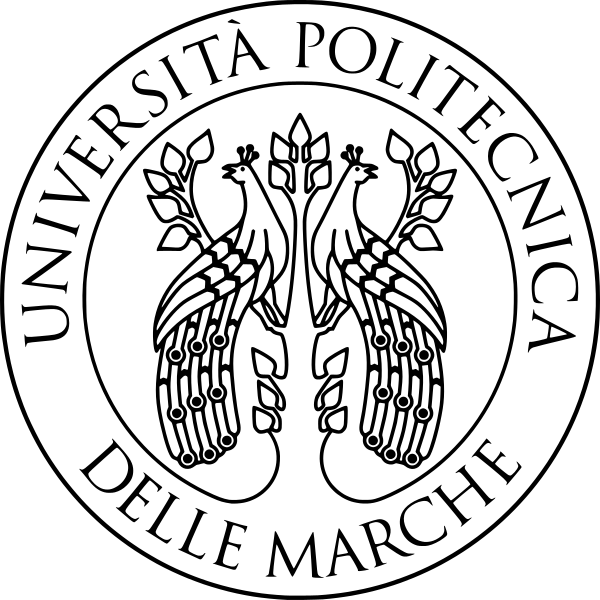
\includegraphics[width=.2\textwidth]{Immagini/univpmlogo}\par\vspace{1cm}
	{\scshape\LARGE Università Politecnica delle Marche\par}
	\vspace{1cm}
	{\scshape\Large Digital Adaptive Circuits And Learning Systems\par}
	\vspace{1.5cm}
	{\huge\bfseries Sound Event Detection con la tecnica del  ``\emph{few-shot learning}''  \par}
	\vspace{2cm}
	{\Large\itshape Matteo Orlandini e Jacopo Pagliuca\par}
	\vfill
	Prof. Stefano \textsc{Squartini}\\
	Dott.ssa Michela \textsc{Cantarini}
	
	\vfill
	
	% Bottom of the page
	{\large \today\par}
\end{titlepage}

\thispagestyle{empty}
\tableofcontents

%\newpage
\setcounter{page}{1}
\section{Introduzione}
\label{section:Introduzione}

\section{Few-shot learning}
\label{section:Few-shot}
(https://www.borealisai.com/en/blog/tutorial-2-few-shot-learning-and-meta-learning-i/)
\subsection{Introduzione}
Gli esseri umani possono riconoscere nuove classi di oggetti da pochissime istanze. Tuttavia, la maggior parte delle tecniche di apprendimento automatico richiedono migliaia di esempi per ottenere prestazioni simili. L'obiettivo dell'apprendimento a breve termine è classificare i nuovi dati dopo aver visto solo pochi esempi di allenamento. All'estremo, potrebbe esserci solo un singolo esempio di ogni classe (one shot learning). In pratica, l'apprendimento a breve termine è utile quando è difficile trovare esempi di training (ad es. casi di una malattia rara) o quando il costo dell'etichettatura dei dati è elevato.

L'apprendimento a pochi colpi viene solitamente studiato utilizzando la classificazione N-way-K-shot. Qui, miriamo a discriminare tra N classi con K esempi di ciascuno. Una tipica dimensione del problema potrebbe essere quella di discriminare tra N=10 classi con solo K=5 campioni da ciascuno da cui allenarsi. Non possiamo addestrare un classificatore usando metodi convenzionali qui; qualsiasi algoritmo di classificazione moderno dipenderà da molti più parametri rispetto agli esempi di addestramento e generalizzerà male.
Se i dati non sono sufficienti per ridurre il problema, una possibile soluzione è acquisire esperienza da altri problemi simili. A tal fine, la maggior parte degli approcci caratterizza l'apprendimento a breve termine con un problema di meta-apprendimento.

\subsection{The meta learning framework}
Nel framework di apprendimento classico, impariamo come classificare dai dati di addestramento e valutiamo i risultati utilizzando i dati di test. Nel quadro del meta-apprendimento, \textit{impariamo come imparare} a classificare in base a una serie di \textit{training task} e valutiamo utilizzando una serie di test task; In altre parole, usiamo un insieme di problemi di classificazione per aiutare a risolvere altri insiemi non correlati.
Qui, ogni attività imita lo scenario few-shot, quindi per la classificazione N-way-K-shot, ogni attività include N classi con K esempi di ciascuno. Questi sono noti come support set per il task e vengono utilizzati per apprendere come risolvere questa task. Inoltre, esistono ulteriori esempi delle stesse classi, note come set di query, utilizzate per valutare le prestazioni del task corrente. Ogni task può essere completamente unico; potremmo non vedere mai le classi di un task in nessuno degli altri. L'idea è che il sistema veda ripetutamente istanze (task) durante l'addestramento che corrispondono alla struttura dell'attività finale di few-shot, ma che contengono classi diverse.
Ad ogni fase del meta-apprendimento, aggiorniamo i parametri del modello in base ad un training task selezionato casualmente. La funzione di loss è determinata dalle prestazioni di classificazione sul set di query del task, in base alla conoscenza acquisita dal relativo set di supporto. Poiché la rete viene sottoposta ad un compito diverso in ogni fase temporale, deve imparare a discriminare le classi di dati in generale, piuttosto che un particolare sottoinsieme di classi.

Per valutare le prestazioni in pochi colpi, utilizziamo una serie di attività di test. Ciascuno contiene solo classi invisibili che non erano in nessuna delle attività di formazione. Per ciascuno, misuriamo le prestazioni sul set di query in base alla conoscenza del loro set di supporto.

\subsection{Approcci al meta-apprendimento}
Gli approcci al meta-apprendimento sono diversi e non c'è consenso sull'approccio migliore. Tuttavia, esistono tre famiglie distinte, ognuna delle quali sfrutta un diverso tipo di conoscenza a priori:
\begin{itemize}
	\item Conoscenze a priori sulla somiglianza: apprendiamo degli embedding nei training task che tendono a separare classi diverse anche quando non sono visibili.
	\item Conoscenze a priori sull'apprendimento: utilizziamo le conoscenze a priori per vincolare l'algoritmo di apprendimento a scegliere parametri che generalizzino bene da pochi esempi.
	\item Conoscenza a priori dei dati: sfruttiamo le conoscenze a priori sulla struttura e la variabilità dei dati e questo ci consente di apprendere modelli praticabili da pochi esempi.
\end{itemize}

\nocite{*}
%Il comando \printbibliography produce la sezione bibliografica con relativi
%titolo e testatina. Per mandarne il relativo titolo nell’indice generale si
%usa l’istruzione:
\printbibliography

\end{document} 